
%(BEGIN_QUESTION)
% Copyright 2006, Tony R. Kuphaldt, released under the Creative Commons Attribution License (v 1.0)
% This means you may do almost anything with this work of mine, so long as you give me proper credit

Suppose we use a thermocouple to measure the temperature of a furnace, a voltmeter to indicate the voltage generated, and we infer furnace temperature from that measured voltage:

$$\includegraphics[width=15.5cm]{i00371x01.eps}$$

Describe what will happen to the voltmeter's indication if the ambient temperature of the instrument room increases while the furnace temperature remains the same, and explain why.

\vskip 10pt

Also, explain what would happen if an inexperienced instrument technician tried to check the calibration of the indicating meter by disconnecting the thermocouple from it and connecting a loop calibrator set to ``Source'' mode like this:

$$\includegraphics[width=15.5cm]{i00371x03.eps}$$

\vskip 20pt \vbox{\hrule \hbox{\strut \vrule{} {\bf Suggestions for Socratic discussion} \vrule} \hrule}

\begin{itemize}
\item{} Suppose a wire broke open in this particular thermocouple circuit.  How would this affect the meter's indication of temperature?
\item{} Suggest a better piece of test equipment for this task than a loop calibrator, and explain how it is supposed to function.
\end{itemize}

\underbar{file i00371}
%(END_QUESTION)





%(BEGIN_ANSWER)

The voltage output by a milliamp calibrator (in Source mode) would likely ruin the sensitive voltmeter indicator, because that indicator is designed to operate on nothing more than tens of {\it millivolts}.  The calibrator likely outputs at least 12 volts in its attempt to force a 4 to 20 mA current through the meter!

\vskip 10pt

{\bf This is a very common way that students have destroyed thermocouple-input instruments in past classes!  A few volts might not seem to harbor any hazards, but it is most definitely destructive to an instrument designed to function on mere millivolt-range signals.}

%(END_ANSWER)





%(BEGIN_NOTES)

If the temperature of the instrument room increases, the voltmeter will indicate a {\it decreased} voltage, leading us to believe that the furnace is cooler than it really is.

\vskip 10pt

Because all complete thermocouple circuits have more than one dissimilar-metal junction, with one junction's generated voltage opposing another, the net voltage measured by any voltmeter in the circuit will be proportional to the {\it difference} in temperature between those opposing junctions:

$$\includegraphics[width=15.5cm]{i00371x02.eps}$$

The voltage output by a milliamp calibrator (in Source mode) would likely ruin the sensitive voltmeter indicator, because that indicator is designed to operate on nothing more than tens of {\it millivolts}.  The calibrator likely outputs at least 12 volts in its attempt to force a 4 to 20 mA current through the meter!

\vskip 10pt

{\bf This is a very common way that students have destroyed thermocouple-input instruments in past classes!  A few volts might not seem to harbor any hazards, but it is most definitely destructive to an instrument designed to function on mere millivolt-range signals.}





\vfil \eject

\noindent
{\bf Prep Quiz:}

Suppose we use a thermocouple to measure the temperature of a furnace, a voltmeter to indicate the voltage generated, and we infer furnace temperature from that measured voltage:

$$\includegraphics[width=15.5cm]{i00371x01.eps}$$

Describe what will happen to the voltmeter's indication if the instrument room becomes warmer while the furnace temperature remains the same.

\vfil \eject

\noindent
{\bf Prep Quiz:}

Suppose we use a thermocouple to measure the temperature of a furnace, a voltmeter to indicate the voltage generated, and we infer furnace temperature from that measured voltage:

$$\includegraphics[width=15.5cm]{i00371x01.eps}$$

Describe what will happen to the voltmeter's indication if the instrument room becomes cooler while the furnace temperature remains the same.


%INDEX% Measurement, temperature: thermocouple

%(END_NOTES)


